% Options for packages loaded elsewhere
% Options for packages loaded elsewhere
\PassOptionsToPackage{unicode}{hyperref}
\PassOptionsToPackage{hyphens}{url}
\PassOptionsToPackage{dvipsnames,svgnames,x11names}{xcolor}
%
\documentclass[
  japanese,
]{beamer}
\usepackage{xcolor}
\usepackage{amsmath,amssymb}
\setcounter{secnumdepth}{-\maxdimen} % remove section numbering
\usepackage{iftex}
\ifPDFTeX
  \usepackage[T1]{fontenc}
  \usepackage[utf8]{inputenc}
  \usepackage{textcomp} % provide euro and other symbols
\else % if luatex or xetex
  \usepackage{unicode-math} % this also loads fontspec
  \defaultfontfeatures{Scale=MatchLowercase}
  \defaultfontfeatures[\rmfamily]{Ligatures=TeX,Scale=1}
\fi
\usepackage{lmodern}
\ifPDFTeX\else
  % xetex/luatex font selection
\fi
% Use upquote if available, for straight quotes in verbatim environments
\IfFileExists{upquote.sty}{\usepackage{upquote}}{}
\IfFileExists{microtype.sty}{% use microtype if available
  \usepackage[]{microtype}
  \UseMicrotypeSet[protrusion]{basicmath} % disable protrusion for tt fonts
}{}
\makeatletter
\@ifundefined{KOMAClassName}{% if non-KOMA class
  \IfFileExists{parskip.sty}{%
    \usepackage{parskip}
  }{% else
    \setlength{\parindent}{0pt}
    \setlength{\parskip}{6pt plus 2pt minus 1pt}}
}{% if KOMA class
  \KOMAoptions{parskip=half}}
\makeatother
% Make \paragraph and \subparagraph free-standing
\makeatletter
\ifx\paragraph\undefined\else
  \let\oldparagraph\paragraph
  \renewcommand{\paragraph}{
    \@ifstar
      \xxxParagraphStar
      \xxxParagraphNoStar
  }
  \newcommand{\xxxParagraphStar}[1]{\oldparagraph*{#1}\mbox{}}
  \newcommand{\xxxParagraphNoStar}[1]{\oldparagraph{#1}\mbox{}}
\fi
\ifx\subparagraph\undefined\else
  \let\oldsubparagraph\subparagraph
  \renewcommand{\subparagraph}{
    \@ifstar
      \xxxSubParagraphStar
      \xxxSubParagraphNoStar
  }
  \newcommand{\xxxSubParagraphStar}[1]{\oldsubparagraph*{#1}\mbox{}}
  \newcommand{\xxxSubParagraphNoStar}[1]{\oldsubparagraph{#1}\mbox{}}
\fi
\makeatother

\usepackage{color}
\usepackage{fancyvrb}
\newcommand{\VerbBar}{|}
\newcommand{\VERB}{\Verb[commandchars=\\\{\}]}
\DefineVerbatimEnvironment{Highlighting}{Verbatim}{commandchars=\\\{\}}
% Add ',fontsize=\small' for more characters per line
\usepackage{framed}
\definecolor{shadecolor}{RGB}{241,243,245}
\newenvironment{Shaded}{\begin{snugshade}}{\end{snugshade}}
\newcommand{\AlertTok}[1]{\textcolor[rgb]{0.68,0.00,0.00}{#1}}
\newcommand{\AnnotationTok}[1]{\textcolor[rgb]{0.37,0.37,0.37}{#1}}
\newcommand{\AttributeTok}[1]{\textcolor[rgb]{0.40,0.45,0.13}{#1}}
\newcommand{\BaseNTok}[1]{\textcolor[rgb]{0.68,0.00,0.00}{#1}}
\newcommand{\BuiltInTok}[1]{\textcolor[rgb]{0.00,0.23,0.31}{#1}}
\newcommand{\CharTok}[1]{\textcolor[rgb]{0.13,0.47,0.30}{#1}}
\newcommand{\CommentTok}[1]{\textcolor[rgb]{0.37,0.37,0.37}{#1}}
\newcommand{\CommentVarTok}[1]{\textcolor[rgb]{0.37,0.37,0.37}{\textit{#1}}}
\newcommand{\ConstantTok}[1]{\textcolor[rgb]{0.56,0.35,0.01}{#1}}
\newcommand{\ControlFlowTok}[1]{\textcolor[rgb]{0.00,0.23,0.31}{\textbf{#1}}}
\newcommand{\DataTypeTok}[1]{\textcolor[rgb]{0.68,0.00,0.00}{#1}}
\newcommand{\DecValTok}[1]{\textcolor[rgb]{0.68,0.00,0.00}{#1}}
\newcommand{\DocumentationTok}[1]{\textcolor[rgb]{0.37,0.37,0.37}{\textit{#1}}}
\newcommand{\ErrorTok}[1]{\textcolor[rgb]{0.68,0.00,0.00}{#1}}
\newcommand{\ExtensionTok}[1]{\textcolor[rgb]{0.00,0.23,0.31}{#1}}
\newcommand{\FloatTok}[1]{\textcolor[rgb]{0.68,0.00,0.00}{#1}}
\newcommand{\FunctionTok}[1]{\textcolor[rgb]{0.28,0.35,0.67}{#1}}
\newcommand{\ImportTok}[1]{\textcolor[rgb]{0.00,0.46,0.62}{#1}}
\newcommand{\InformationTok}[1]{\textcolor[rgb]{0.37,0.37,0.37}{#1}}
\newcommand{\KeywordTok}[1]{\textcolor[rgb]{0.00,0.23,0.31}{\textbf{#1}}}
\newcommand{\NormalTok}[1]{\textcolor[rgb]{0.00,0.23,0.31}{#1}}
\newcommand{\OperatorTok}[1]{\textcolor[rgb]{0.37,0.37,0.37}{#1}}
\newcommand{\OtherTok}[1]{\textcolor[rgb]{0.00,0.23,0.31}{#1}}
\newcommand{\PreprocessorTok}[1]{\textcolor[rgb]{0.68,0.00,0.00}{#1}}
\newcommand{\RegionMarkerTok}[1]{\textcolor[rgb]{0.00,0.23,0.31}{#1}}
\newcommand{\SpecialCharTok}[1]{\textcolor[rgb]{0.37,0.37,0.37}{#1}}
\newcommand{\SpecialStringTok}[1]{\textcolor[rgb]{0.13,0.47,0.30}{#1}}
\newcommand{\StringTok}[1]{\textcolor[rgb]{0.13,0.47,0.30}{#1}}
\newcommand{\VariableTok}[1]{\textcolor[rgb]{0.07,0.07,0.07}{#1}}
\newcommand{\VerbatimStringTok}[1]{\textcolor[rgb]{0.13,0.47,0.30}{#1}}
\newcommand{\WarningTok}[1]{\textcolor[rgb]{0.37,0.37,0.37}{\textit{#1}}}

\usepackage{longtable,booktabs,array}
\usepackage{calc} % for calculating minipage widths
% Correct order of tables after \paragraph or \subparagraph
\usepackage{etoolbox}
\makeatletter
\patchcmd\longtable{\par}{\if@noskipsec\mbox{}\fi\par}{}{}
\makeatother
% Allow footnotes in longtable head/foot
\IfFileExists{footnotehyper.sty}{\usepackage{footnotehyper}}{\usepackage{footnote}}
\makesavenoteenv{longtable}
\usepackage{graphicx}
\makeatletter
\newsavebox\pandoc@box
\newcommand*\pandocbounded[1]{% scales image to fit in text height/width
  \sbox\pandoc@box{#1}%
  \Gscale@div\@tempa{\textheight}{\dimexpr\ht\pandoc@box+\dp\pandoc@box\relax}%
  \Gscale@div\@tempb{\linewidth}{\wd\pandoc@box}%
  \ifdim\@tempb\p@<\@tempa\p@\let\@tempa\@tempb\fi% select the smaller of both
  \ifdim\@tempa\p@<\p@\scalebox{\@tempa}{\usebox\pandoc@box}%
  \else\usebox{\pandoc@box}%
  \fi%
}
% Set default figure placement to htbp
\def\fps@figure{htbp}
\makeatother



\ifLuaTeX
\usepackage[bidi=basic,provide=*]{babel}
\else
\usepackage[bidi=default,provide=*]{babel}
\fi
% get rid of language-specific shorthands (see #6817):
\let\LanguageShortHands\languageshorthands
\def\languageshorthands#1{}


\setlength{\emergencystretch}{3em} % prevent overfull lines

\providecommand{\tightlist}{%
  \setlength{\itemsep}{0pt}\setlength{\parskip}{0pt}}



 


\makeatletter
\@ifpackageloaded{caption}{}{\usepackage{caption}}
\AtBeginDocument{%
\ifdefined\contentsname
  \renewcommand*\contentsname{目次}
\else
  \newcommand\contentsname{目次}
\fi
\ifdefined\listfigurename
  \renewcommand*\listfigurename{図一覧}
\else
  \newcommand\listfigurename{図一覧}
\fi
\ifdefined\listtablename
  \renewcommand*\listtablename{表一覧}
\else
  \newcommand\listtablename{表一覧}
\fi
\ifdefined\figurename
  \renewcommand*\figurename{図}
\else
  \newcommand\figurename{図}
\fi
\ifdefined\tablename
  \renewcommand*\tablename{表}
\else
  \newcommand\tablename{表}
\fi
}
\@ifpackageloaded{float}{}{\usepackage{float}}
\floatstyle{ruled}
\@ifundefined{c@chapter}{\newfloat{codelisting}{h}{lop}}{\newfloat{codelisting}{h}{lop}[chapter]}
\floatname{codelisting}{コード}
\newcommand*\listoflistings{\listof{codelisting}{コード一覧}}
\makeatother
\makeatletter
\makeatother
\makeatletter
\@ifpackageloaded{caption}{}{\usepackage{caption}}
\@ifpackageloaded{subcaption}{}{\usepackage{subcaption}}
\makeatother
\usepackage{bookmark}
\IfFileExists{xurl.sty}{\usepackage{xurl}}{} % add URL line breaks if available
\urlstyle{same}
\hypersetup{
  pdftitle={Quarto × reveal.js 統合デモ},
  pdfauthor={ラボ共有資料},
  pdflang={ja},
  colorlinks=true,
  linkcolor={blue},
  filecolor={Maroon},
  citecolor={Blue},
  urlcolor={Blue},
  pdfcreator={LaTeX via pandoc}}


\title{Quarto × reveal.js 統合デモ}
\author{ラボ共有資料}
\date{2026-02-06}
\begin{document}
\maketitle


\subsection{このデモの目的}\label{ux3053ux306eux30c7ux30e2ux306eux76eeux7684}

\begin{itemize}
\tightlist
\item
  Markdown 1ファイルから reveal.js スライドを生成する
\item
  同じ原稿を PDF にも落とし込んで配布に備える
\item
  再現できるコマンドを残し、研究室の誰でも追従できるようにする
\end{itemize}

ブラウザ登壇を主にしつつ、査読や資料配布でPDFが求められたときの逃げ道を確保しておきたい、という前提を共有。

\subsection{Quarto と reveal.js
の役割分担}\label{quarto-ux3068-reveal.js-ux306eux5f79ux5272ux5206ux62c5}

\begin{itemize}
\tightlist
\item
  \textbf{Quarto} = Markdown
  を多形式に変換する統合ビルドツール(Pandoc・Jupyter を内包)
\item
  \textbf{reveal.js} = ブラウザ上でスライドを描画するプレゼンエンジン
\item
  \texttt{.qmd} 1つで HTML スライドと PDF を両立させる
\end{itemize}

Quarto が「Markdown → reveal.js 構造化
HTML」への変換とオプション注入を行い、reveal.js
が実際のアニメーション・ナビゲーションを提供する。

\subsection{\texorpdfstring{\texttt{.qmd} と \texttt{.md}
の違い}{.qmd と .md の違い}}\label{qmd-ux3068-.md-ux306eux9055ux3044}

\begin{itemize}
\tightlist
\item
  冒頭の \textbf{YAML front matter} で \texttt{format}
  設定・タイトル・言語等を定義
\item
  \texttt{:::\ notes} や \texttt{:::\ \{.columns\}} など \textbf{Pandoc
  fenced divs} が使える
\item
  \texttt{\textasciigrave{}\textasciigrave{}\textasciigrave{}\{python\}}
  のような\textbf{コードチャンク}で実行ブロックを記述可能
\item
  \texttt{.md} より「構造+設定」を厳密に書ける代わりに、YAML 記法や
  fenced div を覚える必要がある
\end{itemize}

\subsection{ディレクトリ構成}\label{ux30c7ux30a3ux30ecux30afux30c8ux30eaux69cbux6210}

\begin{Shaded}
\begin{Highlighting}[]
\NormalTok{demo/}
\NormalTok{├── slides.qmd       \# 原稿(このファイル)}
\NormalTok{├── slides.html      \# reveal.js 版(quarto render {-}{-}to revealjs)}
\NormalTok{├── slides.pdf       \# PDF 版(Chrome ヘッドレス印刷)}
\NormalTok{├── img/             \# 図表ファイル}
\NormalTok{│   ├── figure{-}half.svg}
\NormalTok{│   ├── figure{-}top.svg}
\NormalTok{│   └── figure{-}quarter.svg}
\NormalTok{└── Makefile         \# ワンコマンドビルド}
\end{Highlighting}
\end{Shaded}

\subsection{ワークフロー}\label{ux30efux30fcux30afux30d5ux30edux30fc}

\begin{enumerate}
\def\labelenumi{\arabic{enumi}.}
\tightlist
\item
  \texttt{quarto\ check} で依存関係(Pandoc / LaTeX 等)を確認
\item
  \texttt{quarto\ preview\ slides.qmd} でライブプレビュー
\item
  \texttt{quarto\ render\ slides.qmd\ -\/-to\ revealjs} で HTML 確定
\item
  \texttt{google-chrome\ -\/-headless\ -\/-print-to-pdf} で配布用 PDF
  を生成
\end{enumerate}

\texttt{quarto\ render\ -\/-to\ revealjs} は .qmd の YAML
を読み取り、Pandoc 経由で reveal.js 互換 HTML
を生成するコマンド。\texttt{-\/-to\ pdf} \texttt{-\/-to\ pptx}
など同じ原稿から別形式も作成できる。

\subsection{セクションとサブスライド}\label{ux30bbux30afux30b7ux30e7ux30f3ux3068ux30b5ux30d6ux30b9ux30e9ux30a4ux30c9}

\begin{itemize}
\tightlist
\item
  \texttt{\#\#} 見出しごとに1枚のスライド(水平方向、左右キーで移動)
\item
  同じ \texttt{\#\#} の直後に \texttt{\#\#\#}
  を書くと垂直サブスライドになる(上下キーで移動)
\end{itemize}

\subsubsection{サブスライド
A}\label{ux30b5ux30d6ux30b9ux30e9ux30a4ux30c9-a}

セクション内の1ページ目。

\subsubsection{サブスライド
B}\label{ux30b5ux30d6ux30b9ux30e9ux30a4ux30c9-b}

下矢印で2ページ目へ進む。

\subsection{段階表示
(incremental)}\label{ux6bb5ux968eux8868ux793a-incremental}

\begin{itemize}
\tightlist
\item
  YAML で \texttt{format.revealjs.incremental:\ true}
  と書くとリスト要素が段階表示になる
\item
  ここでは 1 クリックごとに行が表示される
\item
  \texttt{:::\{.incremental\}}
  を本文側に書いて局所的にオンにすることも可能
\end{itemize}

\subsection{embed-resources: true
の効果}\label{embed-resources-true-ux306eux52b9ux679c}

\begin{itemize}
\tightlist
\item
  CSS / JS / 画像を 1 つの HTML にバンドル(Base64
  化してインライン展開)
\item
  ネットワークに接続できない会場やファイル単体配布に便利
\item
  ファイルサイズは大きくなるので、動画は外部ファイルのままが無難
\end{itemize}

\subsection{スピーカーノートの使い方}\label{ux30b9ux30d4ux30fcux30abux30fcux30ceux30fcux30c8ux306eux4f7fux3044ux65b9}

\begin{enumerate}
\def\labelenumi{\arabic{enumi}.}
\tightlist
\item
  本文の後に \texttt{:::\ notes} ブロックを置く
\item
  Markdown で台本を書く(箇条書きも可)
\item
  reveal.js のプレゼンタービュー(\texttt{s}
  キー)で登壇者だけが確認できる
\end{enumerate}

\texttt{quarto\ render\ -\/-to\ pptx} で PowerPoint
出力した場合はノート欄に転記される。特定の読み上げ規格には依存しない。

\subsection{layout: true
による共有背景}\label{layout-true-ux306bux3088ux308bux5171ux6709ux80ccux666f}

\texttt{\{layout="true"\}}
を見出しに付けると、後続サブスライドへ背景・共通要素を継承する。

\subsubsection{レイアウト継承スライド
1}\label{ux30ecux30a4ux30a2ux30a6ux30c8ux7d99ux627fux30b9ux30e9ux30a4ux30c9-1}

\begin{itemize}
\tightlist
\item
  研究ロゴや枠線を複数枚に跨がせたい場合に使う
\item
  同じ背景色や配置を再利用できる
\end{itemize}

\subsubsection{レイアウト継承スライド
2}\label{ux30ecux30a4ux30a2ux30a6ux30c8ux7d99ux627fux30b9ux30e9ux30a4ux30c9-2}

\begin{itemize}
\tightlist
\item
  研究の流れ図などを共通背景として差し込むケースに便利
\end{itemize}

\subsection{カラムレイアウト}\label{ux30abux30e9ux30e0ux30ecux30a4ux30a2ux30a6ux30c8}

\begin{Shaded}
\begin{Highlighting}[]
\ImportTok{import}\NormalTok{ numpy }\ImportTok{as}\NormalTok{ np}
\NormalTok{np.random.seed(}\DecValTok{0}\NormalTok{)}
\BuiltInTok{print}\NormalTok{(np.random.rand(}\DecValTok{3}\NormalTok{))}
\end{Highlighting}
\end{Shaded}

\begin{itemize}
\tightlist
\item
  Quarto のコードブロックは Knitr / Jupyter 実行にも対応
\item
  今回は実行しない静的スライド
\end{itemize}

\subsection{サンプルコード}\label{ux30b5ux30f3ux30d7ux30ebux30b3ux30fcux30c9}

\begin{Shaded}
\begin{Highlighting}[]
\CommentTok{\# HTML スライド生成}
\ExtensionTok{quarto}\NormalTok{ render slides.qmd }\AttributeTok{{-}{-}to}\NormalTok{ revealjs}

\CommentTok{\# Chrome ヘッドレスで PDF 化}
\ExtensionTok{google{-}chrome} \AttributeTok{{-}{-}headless} \AttributeTok{{-}{-}disable{-}gpu} \AttributeTok{{-}{-}no{-}sandbox} \DataTypeTok{\textbackslash{}}
    \AttributeTok{{-}{-}disable{-}dev{-}shm{-}usage} \AttributeTok{{-}{-}print{-}to{-}pdf}\OperatorTok{=}\StringTok{"}\VariableTok{$(}\BuiltInTok{pwd}\VariableTok{)}\StringTok{/slides.pdf"} \DataTypeTok{\textbackslash{}}
    \StringTok{"file://}\VariableTok{$(}\BuiltInTok{pwd}\VariableTok{)}\StringTok{/slides.html?print{-}pdf"}
\end{Highlighting}
\end{Shaded}

\begin{Shaded}
\begin{Highlighting}[]
\CommentTok{\# デモ用: プレースホルダデータを生成}
\ImportTok{import}\NormalTok{ numpy }\ImportTok{as}\NormalTok{ np}
\NormalTok{np.random.seed(}\DecValTok{42}\NormalTok{)}
\NormalTok{noise }\OperatorTok{=}\NormalTok{ np.random.normal(size}\OperatorTok{=}\DecValTok{100}\NormalTok{)}
\NormalTok{trend }\OperatorTok{=}\NormalTok{ np.linspace(}\DecValTok{0}\NormalTok{, }\DecValTok{1}\NormalTok{, }\DecValTok{100}\NormalTok{)}
\NormalTok{data }\OperatorTok{=}\NormalTok{ trend }\OperatorTok{+} \FloatTok{0.2} \OperatorTok{*}\NormalTok{ noise}
\BuiltInTok{print}\NormalTok{(data[:}\DecValTok{5}\NormalTok{])}
\end{Highlighting}
\end{Shaded}

\subsection{図を右半分に配置}\label{ux56f3ux3092ux53f3ux534aux5206ux306bux914dux7f6e}

\begin{itemize}
\tightlist
\item
  2カラム構成にして右側を画像に割り当て
\item
  左カラムに箇条書きや説明を置くと読みやすい
\item
  \texttt{width} 属性でカラム比を微調整可能
\end{itemize}

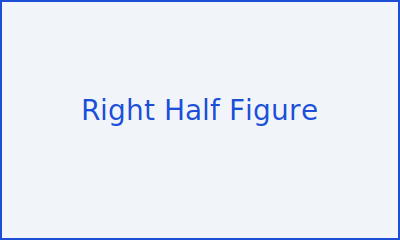
\includegraphics[width=1\linewidth,height=\textheight,keepaspectratio]{slides_files/mediabag/img/figure-half.pdf}

\subsection{図を上半分に配置}\label{ux56f3ux3092ux4e0aux534aux5206ux306bux914dux7f6e}

\begin{figure}[H]

{\centering \pandocbounded{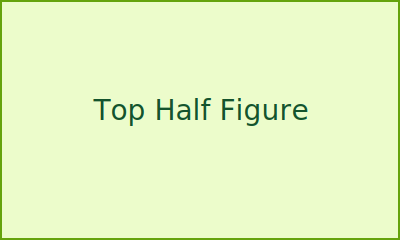
\includegraphics[keepaspectratio]{slides_files/mediabag/img/figure-top.pdf}}

}

\caption{上半分に配置した図}

\end{figure}%

\begin{itemize}
\tightlist
\item
  CSS グリッドで上下2段を作り、上段に図、下段に説明文
\item
  \texttt{height:70vh} で画面高に対する比率を調整
\end{itemize}

:::

\subsection{図を右下 1/4
に固定}\label{ux56f3ux3092ux53f3ux4e0b-14-ux306bux56faux5b9a}

\begin{itemize}
\tightlist
\item
  通常の文章や箇条書きを書いたあと
\item
  \texttt{position:absolute} で右下に小さな図を常時配置
\item
  グラフの抜粋やロゴなど、視覚的な補助として便利
\end{itemize}


\includegraphics[width=1\linewidth,height=\textheight,keepaspectratio]{slides_files/mediabag/img/figure-quarter.pdf}

\subsection{PDF 化の選択肢}\label{pdf-ux5316ux306eux9078ux629eux80a2}

\begin{itemize}
\tightlist
\item
  \textbf{Chrome 印刷}: \texttt{?print-pdf}
  モードで登壇画面と同じ状態をそのまま PDF 化

  \begin{itemize}
  \tightlist
  \item
    \texttt{-\/-no-sandbox\ -\/-disable-dev-shm-usage} は CI
    でも安定する定番フラグ
  \end{itemize}
\item
  \textbf{LaTeX}: \texttt{quarto\ render\ slides.qmd\ -\/-to\ pdf} で
  Beamer ベースの PDF を生成(要 TeX 環境)
\end{itemize}

reveal.js の \texttt{?print-pdf}
は公式ルートなので基本は安定。段階表示の一括表示には
\texttt{pdfSeparateFragments:\ true} を組み合わせる。

\subsection{まとめ}\label{ux307eux3068ux3081}

\begin{itemize}
\tightlist
\item
  Markdown で台本を集中管理し、出力形式は Quarto に任せる
\item
  reveal.js を登壇用、Chrome PDF を配布用という役割分担で破綻を防ぐ
\item
  必要に応じて \texttt{format.pdf}(Beamer)や
  \texttt{-\/-to\ pptx}(PowerPoint)を併産
\item
  \texttt{quarto\ render} を CI
  に組み込めば配布忘れ・崩れを早期検知できる
\end{itemize}

CI 例: GitHub Actions で \texttt{quarto\ render} →
\texttt{google-chrome\ -\/-headless\ -\/-print-to-pdf}
を走らせ、slides.html と slides.pdf をアーティファクト化。




\end{document}
